\chapter{How to use the Dynamic Pipeline Haskell Library}
\section{Objective}
In this section it will be explined the steps to given a dynamic pipeline algorithm, how to implement it using the Haskell library. 
First of all it is necessary to have in mind the structure of the pipeline and the logic of the algorithm.
For better explanation, I will be using a toy problem to illustrate the steps.
I will be using, as said previously, the word counting problem: given a list of words (like a text file or a book), count the number of times each word appears in the list.

\section{Preliminaries}
First of all, it is necessary to design the pipeline structure and our algorithm logic. 
For all dynamic pipeline, we need to define the following concepts:
\begin{itemize} 
    \item \textbf{Source:} Here it is defined how the data will be read and how it will be sent to the pipeline.
    \item \textbf{Generator:} Here it is defined when a filter is generated and which data processes.
    \item \textbf{Sink:} Here it is defined how the data will be received from the pipeline and how it will be written.
\end{itemize}

Now, let's try to define the structure of the pipeline for the word counting problem.
Our input is a chain of caracters that form words and we want to output all unique words folowed by the number of times they appear in the input. \\
\begin{figure}[H]
    \centering
    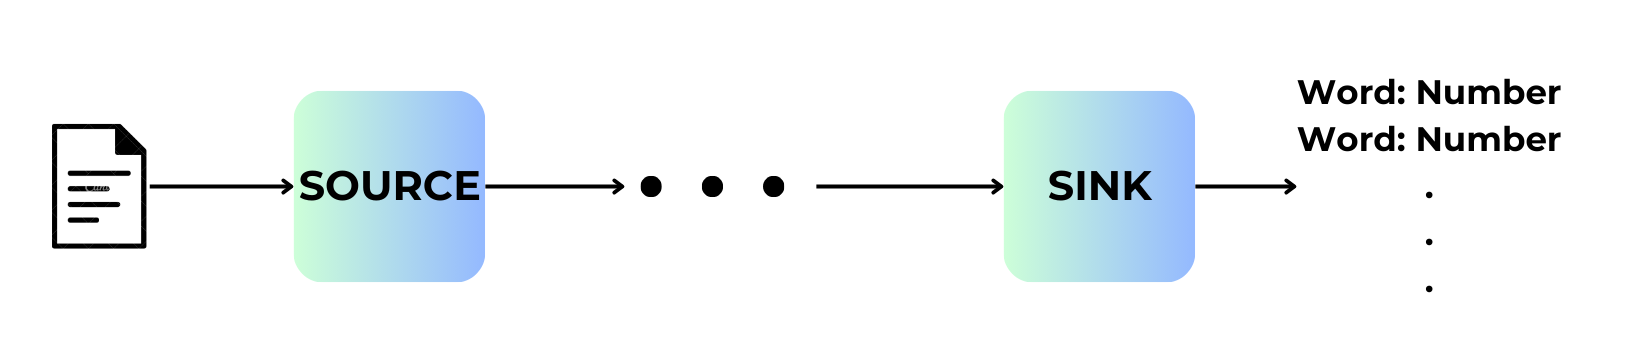
\includegraphics[width=1\textwidth]{DP1.png}
    \caption{First Dynamic Pipeline scheme}
    \label{fig:DP1}
\end{figure}

Now we need to define whichs data types the pipeline will use. 
As we are reading caracters and we are procecing words we are going to use the standard Haskell types: Char and [Char] for characters and words, respectively.
Also we need to keep track of the number of times each word appears, so we will be using a tuple ([Char], Int) to represent the word and the number of times it appears.
So the source needs to read the data, get the words and send them to the pipeline as a list of tuples. 
\begin{figure}[H]
    \centering
    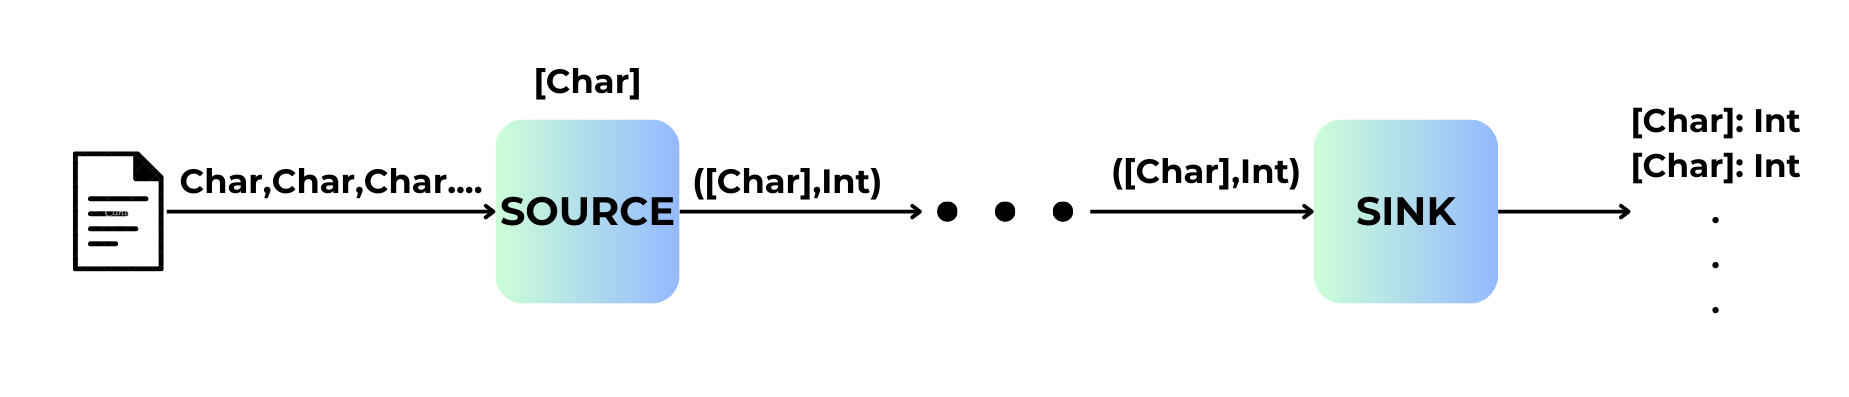
\includegraphics[width=1\textwidth]{DP2.png}
    \caption{Dynamic Pipeline scheme with data types}
    \label{fig:DP2}
\end{figure}

At this point we can start to design the logic of the algorithm.
In our initial state we have just the source, the sink and the generator, so the first thing that we need to decide is, for every data that the generator reads, when it will let the data pass to the sink.
This is because in front of the generator there will be a series of filters processing the data.
Perhaps sometimes it will receive data directly from the input, either modified data or data emitted by filters.
Looking our problem, we see that we do not want to let pass all the data, but we do want to let it pass sometimes.
As we explained at the beginning of this work, the data can be infinite and we want to have a mechanism to be able to print responses throughout the execution.
That is why we have to be able to differentiate between when it is a "normal" data, so we should not let it pass and when it is a response, in order to pass it.
The solution that I have decided to use is based on the fact that for each word we have its word counter, therefore, when a data comes that is a response, the counter will be at least 1.
This allows us make the source to initialize the tuple with ([Char],0), so when the generator receives a tuple with this shape it knows that it is input data.
\begin{figure}[H]
    \centering
    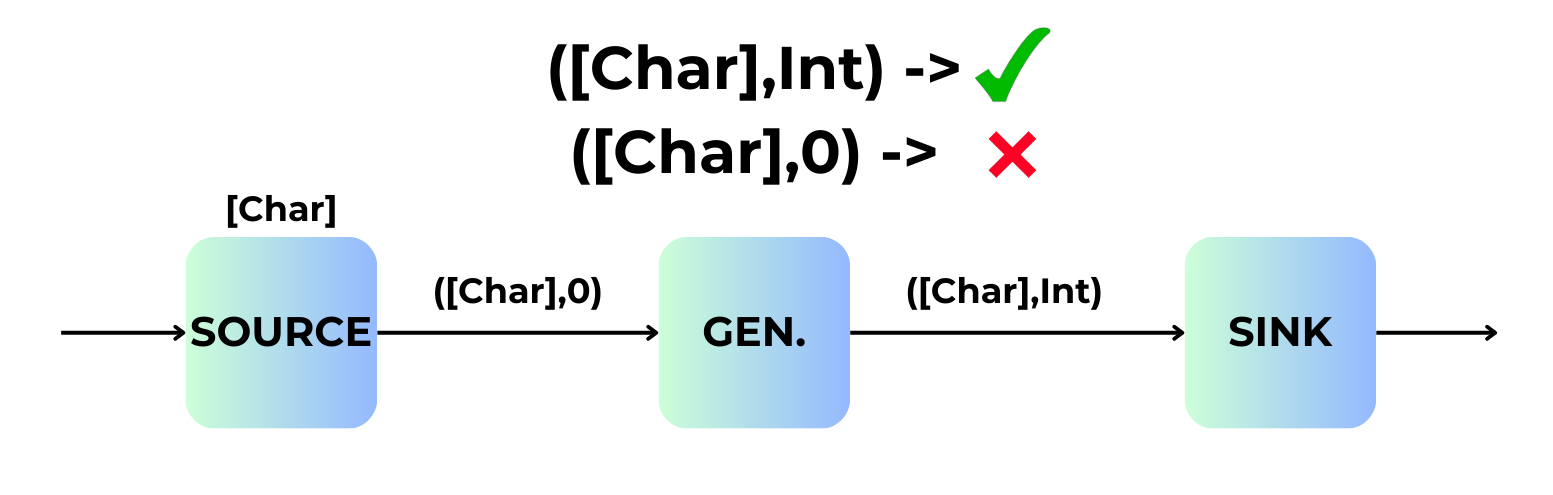
\includegraphics[width=1\textwidth]{DP3.png}
    \caption{Dynamic Pipeline scheme with generator logic for letting pass the words}
    \label{fig:DP3}
\end{figure}
The next step is decide when the generator will emit a filter.
But before that, we need to decide more or less how the filter will be.
Filters acts similar to the others stages: it receives data, it can process it and it can emit data.
A characteristic of each filter is that they have a interal parameter which can be used for the process.
So, with all this in mind, we can make each filter responsible for counting a single word, so that if it receives a word that is not its own, it simply lets it pass.
On the other hand, if it receives a word that matches its parameter, it will add it to its count and will not let it continue passing.
With this filter scheme we can get each one to be in charge of a different word, so we would need to generate a filter for each unique word.
\\

Now we can define when the generator will emit a filter.
The generator will emit a filter each time it recives a new word, and because once a filter is generated for a word, it will not allow more of that word to pass.
All the data (other than results) that the generator reads will be new words and a filter must be generated.
In other words, if the generator recives a tuple with ([Char],0) it will generate a filter. 
\\

We have all set except for for few details.
We need to define how the generator will initialize the filter parameter. 
Since the parameter needs to know which word it controls and how many times it appears, it seems logical to use the ([Char],Int) tuple again.
So the generator will initialize the filter parameter with the tuple that it received from the source, but changing the counter to 1 (because it is the first time that the word appears).
Last but not least, we have to define how to indicate to the pipeline that we want to receive a response in the output (for the incremental behavior).
To do this, what we can do is try to introduce data into the stream that indicates that we should return the response.
We can use a piece of data which does not represent any word, for example the character ".".
In this way, every time a filter receives a tuple (".",Int), it must pass through the pipeline its parameter (which will contain the count) and also the point, so that the rest of the filters repeat the process.
\begin{figure}[H]
    \centering
    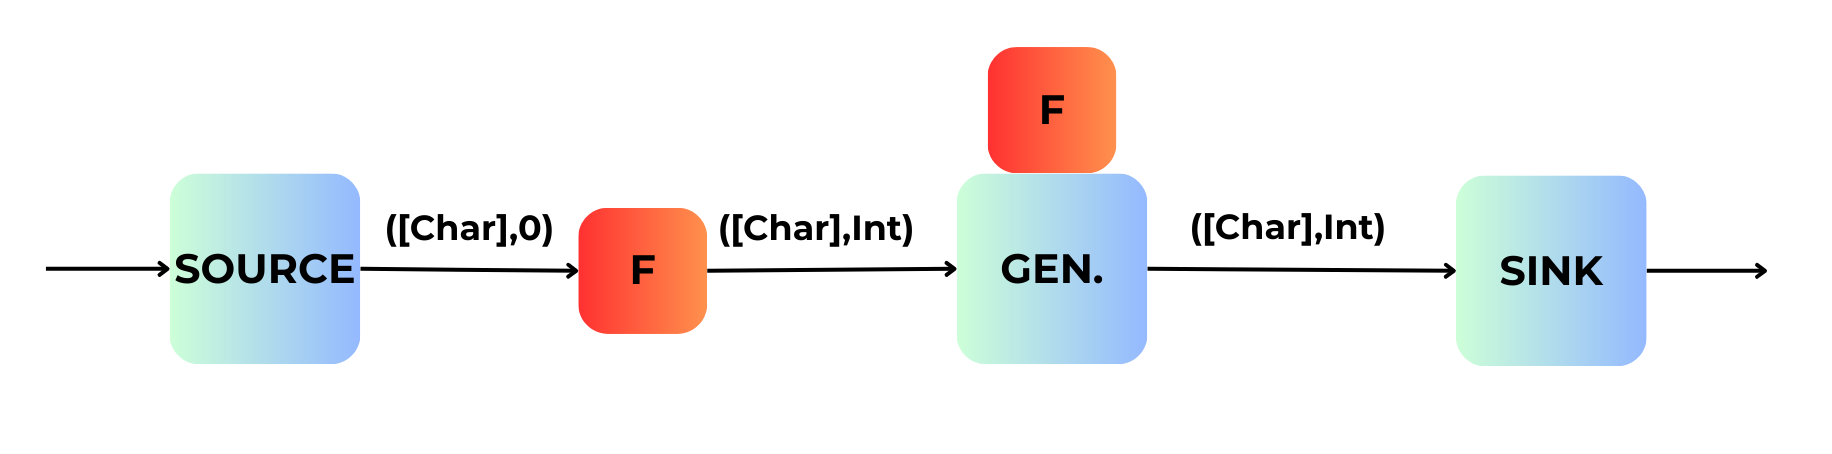
\includegraphics[width=1\textwidth]{DP4.png}
    \caption{Example of a Dynamic Pipeline with one filter generated}
    \label{fig:DP4}
\end{figure}

\section{Example}
Lets make a quick example to illustrate all the concepts explained above.
We will use the following input: ["cat","dog","cat","bird",".","dog","."]
This is the initial state of the pipeline:
\begin{figure}[H]
    \centering
    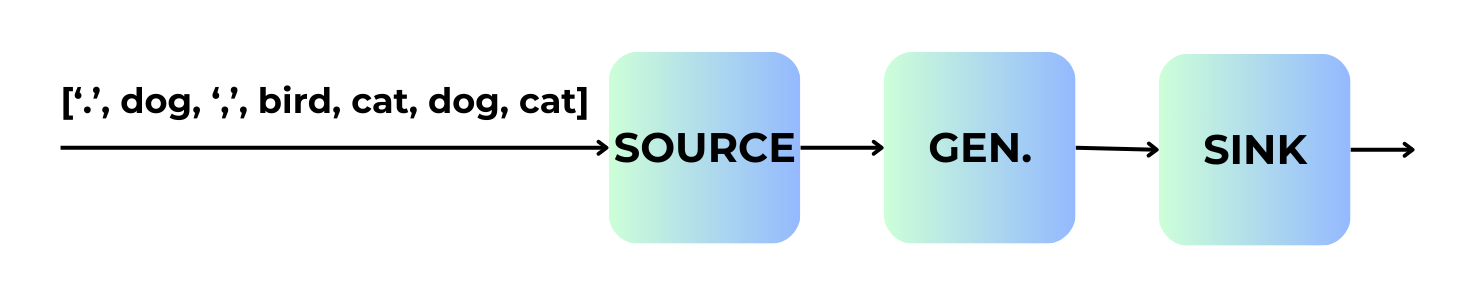
\includegraphics[width=1\textwidth]{DP5.png}
    \caption{Initial state of the Dynamic Pipeline}
    \label{fig:DP5}
\end{figure}

The first word that will be processed is "cat". 
Here is the state of the pipeline after the first word is processed:
\begin{figure}[H]
    \centering
    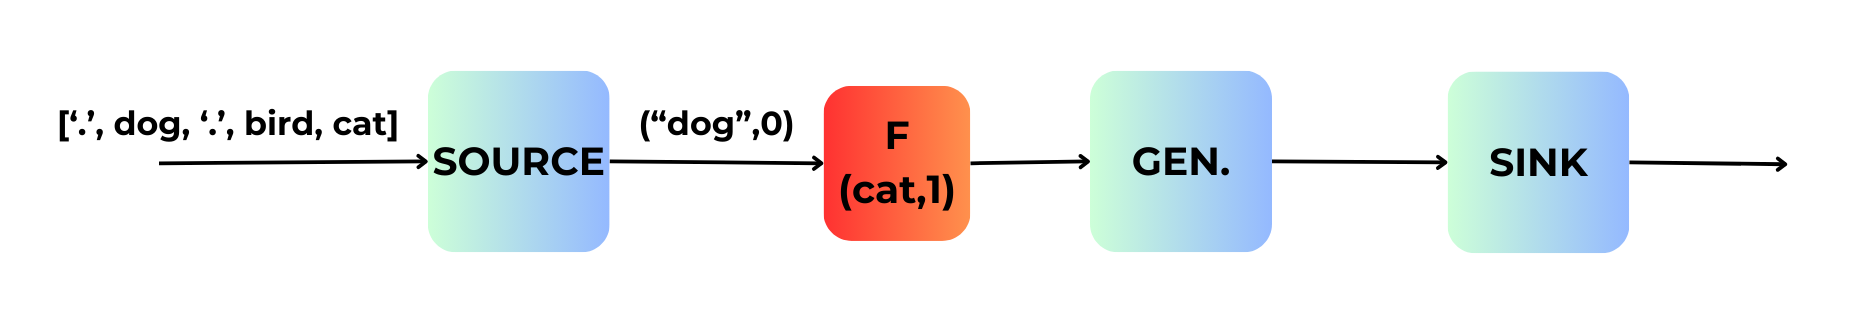
\includegraphics[width=1\textwidth]{DP6.png}
    \caption{Dynamic Pipeline state after the process of the first word}
    \label{fig:DP6}
\end{figure}

If we keep processing the input before we reach the first ".", we will have the following state:
\begin{figure}[H]
    \centering
    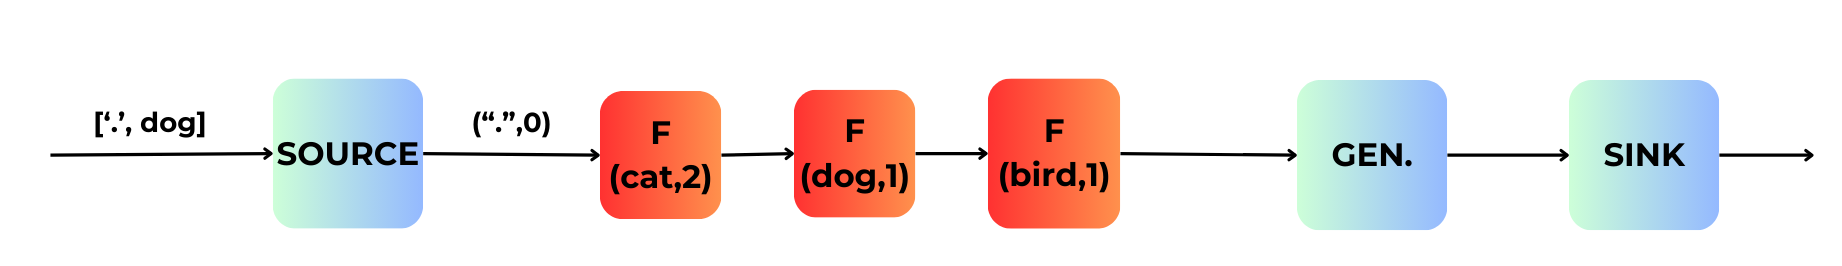
\includegraphics[width=1\textwidth]{DP7.png}
    \caption{Dynamic Pipeline state after reading ["cat","dog","cat","bird"]}
    \label{fig:DP7}
\end{figure}

After reading the ".", the generator will let pass the tuples that the counter is not 0 leaving us with:
\begin{figure}[H]
    \centering
    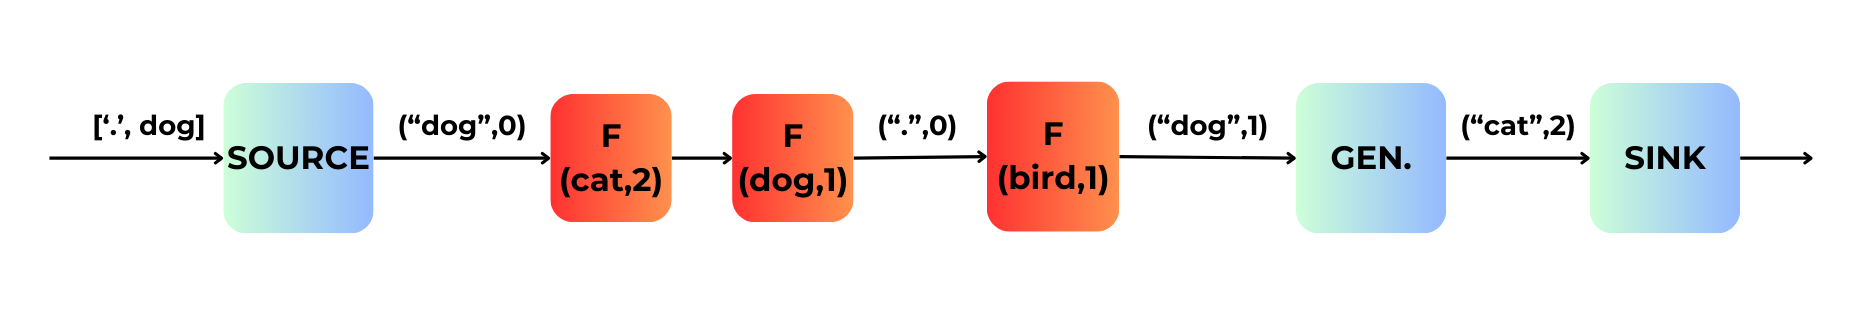
\includegraphics[width=1\textwidth]{DP8.png}
    \caption{Dynamic Pipeline state after reading the first "."}
    \label{fig:DP8}
\end{figure}

The generator readed the tuple ("cat",2) and let it pass to the sink (without generating a filter, because the counter is not 0). 
If we finish all the input we will have the following final state:
\begin{figure}[H]
    \centering
    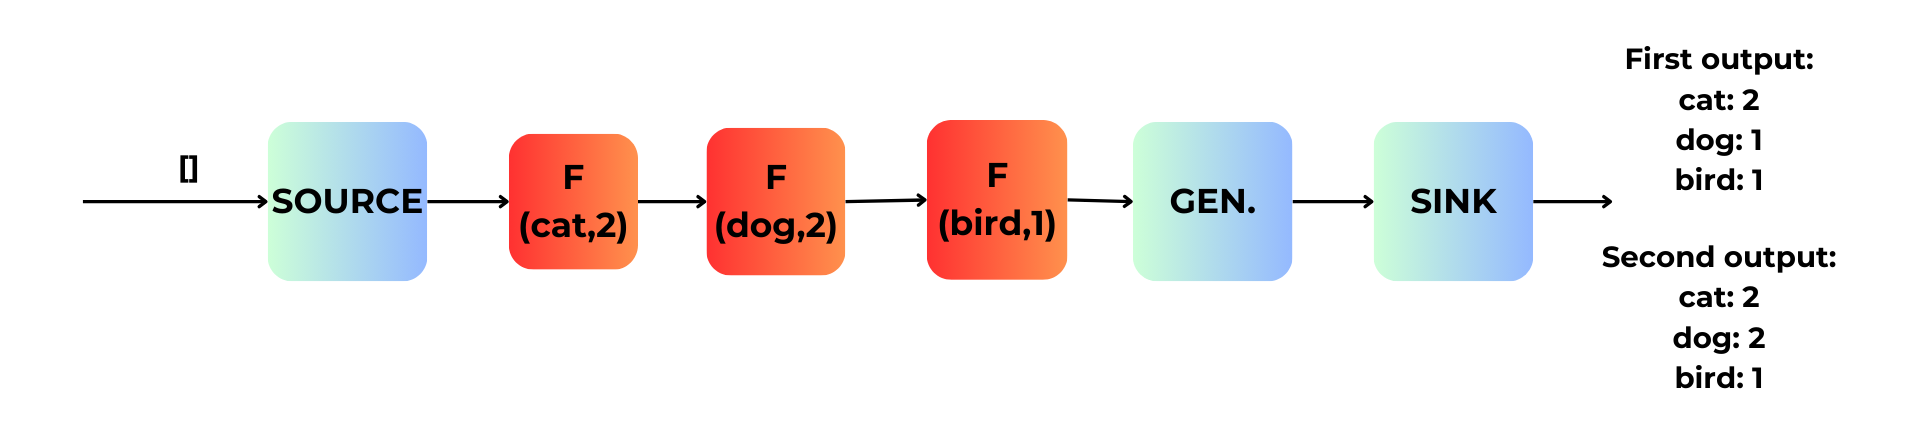
\includegraphics[width=1\textwidth]{DP9.png}
    \caption{Final state of the Dynamic Pipeline}
    \label{fig:DP9}
\end{figure}
\section{Implementation}
Now we designed the pipeline structure and the logic of the algorithm, we can start to implement it using the Haskell library. 
\subsection{Defining the functions}
\subsubsection{Dynamic pipeline data type}
If we check the library, almost all functions make use of a dpDefinition, which is a type that we define representing the structure of the pipeline. 
The tools for defining it provided by the library are the following:

\begin{figure}[H]
    \centering
    \begin{tabular}{c}
        \begin{lstlisting}[escapeinside={(*}{*)}]
        data Sink
        data Generator (a :: Type), a (*$\sim$*) Channel
        data Source (a :: Type), a (*$\sim$*) Channel
        data Channel (a :: Type), a (*$\sim$*) (Type :<+> Type :<+> ... :<+> Eof)
        data DynamicPipeline dpDefinition filterState filterParam st, 
            dpDefinition (*$\sim$*) Source (Channel ..) :=> Generator (Channel ..) :=> Sink
        data a :=> b, a & b (*$\sim$*) Stage
        \end{lstlisting}
    \end{tabular}
    \caption{Data types provided by the library}
    \label{fig:DP10}
\end{figure}

We can see that it provides the data type for all the stages, so lets apply the structure that we designed to the library. 

\begin{figure}[H]
    \centering
    \begin{tabular}{c}
        \begin{lstlisting}[escapeinside={(*}{*)}]
        type DP = Source (Channel (([Char],Int) :<+> Eof)) :=> Generator (Channel (([Char],Int):<+> Eof)) :=> Sink
        \end{lstlisting}
    \end{tabular}
    \caption{Dynamic pipeline type definition}
    \label{fig:DP11}
\end{figure}

As said before, we define the data types that will flow through the pipeline and asign them to the stages. 

\subsubsection{Building the DP}
The next step is building the dynamic pipeline:

\begin{figure}[H]
    \centering
    \begin{tabular}{c}
        \begin{lstlisting}[escapeinside={(*}{*)}]
        mkDP :: forall dpDefinition filterState st . . .
        => Stage (WithSource dpDefinition (DP st))	
        -> GeneratorStage dpDefinition filterState filterParam st	 
        -> Stage (WithSink dpDefinition (DP st))	
        -> DP st ()
        \end{lstlisting}
    \end{tabular}
    \caption{mkDP function definition}
    \label{fig:DP12}
\end{figure}

This functions is smart constructor for the dynamic pipeline. 
If we translate this definition into words, we can see that it receives the definition and the stages of the pipeline and returns the dynamic pipeline.
So we need to define each stage of the pipeline and then use this function to build the dynamic pipeline.

\begin{figure}[H]
    \centering
    \begin{tabular}{c}
        \begin{lstlisting}[escapeinside={(*}{*)}]
        dp' :: DP s ()
        dp' = mkDP @DPExample source' generator' sink'
        \end{lstlisting}
    \end{tabular}
    \caption{Definition of custom function dp'}
    \label{fig:DP13}
\end{figure}

\subsubsection{Building the Source}
The first stage that we are going to define is the source.
The library also provide us with a combinator to build a source stage:

\begin{figure}[H]
    \centering
    \begin{tabular}{c}
        \begin{lstlisting}[escapeinside={(*}{*)}]
        withSource :: forall (dpDefinition :: Type) st. WithSource dpDefinition (DP st)    
        -> Stage (WithSource dpDefinition (DP st))
        \end{lstlisting}
    \end{tabular}
    \caption{Source stage combinator}
    \label{fig:DP14}
\end{figure}

Explined into words, we just need to provide the pipeline definition and a function reads some data and populates de pipeline

\begin{figure}[H]
    \centering
    \begin{tabular}{c}
        \begin{lstlisting}[escapeinside={(*}{*)}]
        source' :: Stage (WriteChannel (ByteString,Int) -> DP s ())
        source' = withSource @DPExample populateSource'

        dp' :: DP s ()
        dp' = mkDP @DPExample source' generator' sink'           
        \end{lstlisting}
    \end{tabular}
    \caption{source' function added to definitions}
    \label{fig:DP15}
\end{figure}

\subsubsection{Building the Sink}
Next stage is the sink, as is more simple. 
The library provides us with a combinator to build a sink stage:

\begin{figure}[H]
    \centering
    \begin{tabular}{c}
        \begin{lstlisting}[escapeinside={(*}{*)}]
        withSinkSource :: forall (dpDefinition :: Type) st. WithSink dpDefinition (DP st)	  
        -> Stage (WithSink dpDefinition (DP st))
        \end{lstlisting}
    \end{tabular}
    \caption{Sink stage combinator}
    \label{fig:DP16}
\end{figure}

Similar to the source, we just need to provide the pipeline definition and a function that reads data form the pipeline and outputs it. 

\begin{figure}[H]
    \centering
    \begin{tabular}{c}
        \begin{lstlisting}[escapeinside={(*}{*)}]
        source' :: Stage (WriteChannel (ByteString,Int) -> DP s ())
        source' = withSource @DP populateSource'

        sink' :: Stage (ReadChannel (ByteString,Int) -> DP s ())
        sink' = withSink @DP outputSink'

        dp' :: DP s ()
        dp' = mkDP @DPExample source' generator' sink'           
        \end{lstlisting}
    \end{tabular}
    \caption{sink' function added to definitions}
    \label{fig:DP17}
\end{figure}

\subsubsection{Building the Generator}
The generator is the most complex stage to build, because we need to define the filters and define the logic of the generator. 
The library provides us with both a smart constructor and a combinator to build the generator stage: 

\begin{figure}[H]
    \centering
    \begin{tabular}{c}
        \begin{lstlisting}[escapeinside={(*}{*)}]
        mkGeneratorSource :: Stage (WithGenerator dpDefinition (Filter dpDefinition filterState filterParam st) (DP st))
        -> Filter dpDefinition filterState filterParam st	
        -> GeneratorStage dpDefinition filterState filterParam st 
        
        withGeneratorSource :: forall (dpDefinition :: Type) (filter :: Type) st. WithGenerator dpDefinition filter (DP st)	
        -> Stage (WithGenerator dpDefinition filter (DP st))
        \end{lstlisting}
    \end{tabular}
    \caption{Generator smart constructor and combinator}
    \label{fig:DP18}
\end{figure}

Seems dificult to understand, but combining this 2 functions with the pipeline definition, the generator logic and a filter template we can build the generator stage. 
Here is the structure to follow to build the generator stage: 

\begin{figure}[H]
    \centering
    \begin{tabular}{c}
        \begin{lstlisting}[escapeinside={(*}{*)}]
        source' :: Stage (WriteChannel (ByteString,Int) -> DP s ())
        source' = withSource @DP populateSource'

        generator' :: GeneratorStage DPExample (ByteString,Int) (ByteString,Int) s
        generator' = mkGenerator withGenerator @DP genLogic'

        sink' :: Stage (ReadChannel (ByteString,Int) -> DP s ())
        sink' = withSink @DP outputSink'

        dp' :: DP s ()
        dp' = mkDP @DPExample source' generator' sink'  
        \end{lstlisting}
    \end{tabular}
    \caption{generator' function added to definitions}
    \label{fig:DP19}
\end{figure}

\subsubsection{Summary} 
We have defined all stages of the pipeline and all the functions needed to build the dynamic pipeline. 

\subsection{Implementinc functions}
We have all defined so we need to implement the diferent functions acording to what we defined previously. 
\subsubsection{Source stage}
For the source we need to define the populateSource' function. 
This function will take a WriteChannel and will write the data to the pipeline. 
The library provides us with some functions to do this: 

\begin{figure}[H]
    \centering
    \begin{tabular}{c}
        \begin{lstlisting}[escapeinside={(*}{*)}]
            unfoldMSource :: forall m a b. MonadIO m	 
            => m a	
            -> (a -> b)	
            -> m Bool	
            -> WriteChannel b	
            -> m ()

            unfoldFileSource :: MonadIO m	 
            => FilePath	
            -> WriteChannel b	
            -> (ByteString -> b)	
            -> m () 
            
            unfoldT :: (MonadIO m, Foldable t) 
            => t a 
            -> WriteChannel b 
            -> (a -> b) 
            -> m ()
        \end{lstlisting}
    \end{tabular}
    \caption{Functions to populate a WriteChannel}
    \label{fig:DP20}
\end{figure}

This 3 functions populates a WriteChannel taking data from diferent inputs. 
For this example lets take the unfoldT function, because allow us to use Foldable (like lists or sets) as input. 

\begin{figure}[H]
    \centering
    \begin{tabular}{c}
        \begin{lstlisting}[escapeinside={(*}{*)}]            
            populateSource' :: WriteChannel b -> m ()
            populateSource' c = unfoldT input c convert 
        \end{lstlisting}
    \end{tabular}
    \caption{populateSource' definition}
    \label{fig:DP21}
\end{figure}

We just need to provide de input (that can be whatever Foldable) and the convert function, that is a function that convert the data type from the input to the WriteChannel. 
Remembering the data types that we defined for the pipeline, we need to convert the input [Char] to a ([Char],0) tuple. 
So all defined, the populateSource' function will be: 

\begin{figure}[H]
    \centering
    \begin{tabular}{c}
        \begin{lstlisting}[escapeinside={(*}{*)}
            input:: [Char]
            input = [ . . .]

            convert :: Char -> ([Char],Int)
            convert w = (w,0)

            populateSource' :: WriteChannel b -> m ()
            populateSource' channel = unfoldT input channel convert 
        \end{lstlisting}
    \end{tabular}
    \caption{populateSource' definition with input and convert functions}
    \label{fig:DP22}
\end{figure}

\subsubsection{Sink stage}
For the sink we need to define the outputSink' function. 
This function will take a ReadChannel and will output the data.
Similar to source stage, the library provides us with some functions to do this: 

\begin{figure}[H]
    \centering
    \begin{tabular}{c}
        \begin{lstlisting}[escapeinside={(*}{*)}]
            foldM_ :: MonadIO m	 
            => ReadChannel a	
            -> (a -> m ())	
            -> m ()
        \end{lstlisting}
    \end{tabular}
    \caption{Functions to read a ReadChannel}
    \label{fig:DP23}
\end{figure}

Now we just have one function, so lets use it: 

\begin{figure}[H]
    \centering
    \begin{tabular}{c}
        \begin{lstlisting}[escapeinside={(*}{*)}]
            outputSink' :: ReadChannel b -> m ()
            outputSink' c = foldM_ c transform
        \end{lstlisting}
    \end{tabular}
    \caption{outputSink' definition}
    \label{fig:DP23}
\end{figure}

Similiar to the source stage, we need to define the transform function that will convert the data from the ReadChannel to the output. 
For this example, we will just print out the data to the console.

\begin{figure}[H]
    \centering
    \begin{tabular}{c}
        \begin{lstlisting}[escapeinside={(*}{*)}]
            transform :: ([Char],Int) -> m ()
            transform (w,c) = putStrLn $ w ++ ": " ++ show c

            outputSink' :: ReadChannel b -> m ()
            outputSink' c = foldM_ c transform
        \end{lstlisting}
    \end{tabular}
    \caption{outputSink' definition with transform function}
    \label{fig:DP24}
\end{figure}

\subsubsection{Generator stage}
For this stage we do a 
